\newpage
\index{QGIS Processing Framework}
\section{QGIS Processing Framework}
\nocite{pf:www}


\begin{center}
		
\includegraphics[scale=0.30]{pictures/qgis_pf}
\end{center}

QGIS Processing Framework vznikl v rámci projektu \footnotemark{GSoC 2011} \footnotetext{Google Summer of Code. Projekt společnosti Google na podporu studentu. více na http://code.google.com/soc/}. Student Camilo Polymeris z univerzity Universidad de Concepción si kladl za cíl napsat obecný framework, do kterého budou zapadat všechny moduly všech pluginů QGISu a každý modul bude možné použít buď samostatně nebo spojovat s jinými.

V době psaní této práce byla na světě první verze Processing Frameworku a vše nasvědčovalo tomu, že práce na frameworku budou pokračovat a nástroje v Processing Frameworku budou přibývat. Existovala totiž pouze částečná  podpora pro funkce z SAGA GIS a plugin zpřístupňující funkce \index{Orfeo Toolbox, OTB} Orfeo Toolboxu (OTB). Orfeo Toolbox je svobodný software poskytující nástroje pro zpracování snímku z \index{DPZ, dálkový průzkum Země} dálkového průzkumu Země.

V době mého připojení k QGIS Processing Frameworku byl projekt na začátku. Pro seznámení s projektem jsem přepsal Processing Manager (toolbox) z QTreeWidget do MVC architektury.

Processing Manager je část QGIS Processing Frameworku, která zpřístupňuje všechny moduly dostupné skrze QGIS Processing Framework z jednoho místa. Jedná se o panel se seznamem modulů, které jsou rozděleny podle tagů do různých skupin (například 'raster', 'hydrology'). Každý modul obsahuje seznam tagů, které napovídají, k čemu daný modul slouží. Uživatel může najít hledaný modul prohledáváním samotného stromu, či využít vyhledávací okénko v horní části panelu. Processing Manager prohledává tagy daného modulu a jeho název. Modul obsahuje dále popis, ale protože se tagy generují z tohoto popisu, nemá cenu popis procházet \figurename \ref{pf:pm}.

\begin{figure}
	\centering
	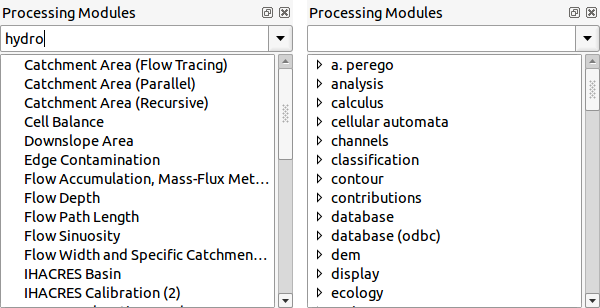
\includegraphics[scale=0.5]{pictures/pf/processing_manager_small}
	\caption{QGIS Processing Framework - Processing Manager}
  	\label{pf:pm}
\end{figure}

{\color{red}Dostupnost skrze pythoní konzoli v QGISU. Načítání modulu, nastavování parametrů, spuštění. takže asi zase malé tabulky - metody a atributy Modulu, Parametru.}

%%%%%%%%%%%%%%%%%%%
%%% SAGA Plugin %%%
%%%%%%%%%%%%%%%%%%%

\subsection{SAGA Plugin}
SAGA Plugin vznikl v rámci stejného projektu Camila Polymeris pro GSoC 2011. Měl zpřístupňovat funkce programu SAGA GIS pomocí jeho API uživatelům Quantum GIS. Na stránkách projektu [\cite{pf:supportedModules}] se deklaruje, že by mělo být podporováno 170 modulů z celkových 425. Toto číslo vychází z předpokladu, že moduly, u kterých jsou všechny vstupní i výstupní parametry podporovány, pracují správně. Podporované parametry SAGA GIS a jejich reprezentace v Processing Frameworku \ref{tab:saga_parameters}. Parametry SAGA GIS, které nejsou podporované Processing Frameworkem$:$ \textit{Table field, Data Object, Grid list, Table, Node, Shape list, Parameters, Point Cloud, TIN, Static table, Table list, Color, TIN list a Colors}. Dále nejsou podporované interaktivní moduly. Bohužel ale nebyl plugin plně dokončen a skutečný počet správně pracujících pluginů není roven 170. \\

\begin{table}	
	\centering
	\begin{tabular}{|c|c|}
		\hline
		\textbf{SAGA parametr} & \textbf{PF Parameter} \\
		\hline
		\hline
		Int & \multirow{3}{*}{NumericParameter}\\
		Double & \\
		Degree & \\
		\hline				
		Range & RangeParameter\\	
		\hline
		Bool & BooleanParameter\\		
		\hline
		String & \multirow{2}{*}{StringParameter}\\
		Text & \\
		\hline
		Chioce & ChoiceParameter\\
		\hline
		FilePath & PathParameter\\
		\hline
		Shapes & VectorLayerParameter\\
		\hline
		Grid & RasterLayerParameter\\		
		\hline	
	\end{tabular}
	\caption{parametry SAGA GIS podporované Processing Frameworkem}
	\label{tab:saga_parameters}
\end{table}


%%%%%%%%%%%%%%%%%%%%%%%%%%%%
%%% Psaní pluginu pro PF %%%
%%%%%%%%%%%%%%%%%%%%%%%%%%%%

\subsection{Psaní pluginu pro PF}

QGIS Processing Framework funguje tak, že si každý může při psaní pluginu pro QGIS může při dodržení pár pravidel \textit{"zaregistrovat"} zaregistrovat svůj modul do frameworku. 

Každý plugin může mít několik vstupních a výstupních parametrů. V současné době dovoluje framework uživateli použít parametry \ref{tab:pf_parametry}.

\begin{table}	
	\centering
	\begin{tabular}{|c|c|c|}
		\hline
		\textbf{parametr} & \textbf{popis} & \textbf{grafická reprezentace}\\
		\hline
		\hline
		NumericParameter & číslo & QSpinBox\\
		\hline
		RangeParameter & dvojice číselných hodnot & pár QSpinBox\\	
		\hline
		BooleanParameter & boolean & QCheckBox\\		
		\hline
		\multirow{2}{*}{ChoiceParameter} & seznam možností & \multirow{2}{*}{QComboBox}\\
		& např. vrstev, metod & \\
		\hline
		StringParameter & textový řetězec & QLineEdit \\
		\hline
		PathParameter & cesta k souboru & QLineEdit + QPushButton \\
		\hline
		\multirow{2}{*}{VectorLayerParameter} & \multirow{2}{*}{QgsVectorLayer} & QComboBox s registrovanými \\
		& & vektorovými vrstvami\\
		\hline
		\multirow{2}{*}{RasterLayerParameter} & \multirow{2}{*}{QgsRasterLayer} & QComboBox s registrovanými \\
		& & rastrovými vrstvami\\		
		\hline	
	\end{tabular}
	\caption{parametry podporované Processing Frameworkem}
	\label{tab:pf_parametry}
\end{table}

Obr. Dialogového okna

%%%%%%%%%%%%%%%%%%
%%% Conclusion %%%
%%%%%%%%%%%%%%%%%%

\subsection{Závěr}

Chtělo by to vyřešit vstupní vrstvy aby například rastrová vrstva zadaná jako PathParameter byla kompatibilní s parametrem RasterLayerParameter. Dát vývojáři pluginu možnost dát uživateli možnost zadat vrstvu buď pomocí cesty nebo výběrem z jich načtených vrstev. Dát uživateli obě možnosti.

Je napsán OTB Plugin pro zpracování družicových snímků a rozepsán SAGA Plugin s podporou několika pluginů z SAGA GIS.

Camilo Polymeris měl v plánu pokračovat na projektu v rámci GSoC 2012, ale po objevení frameworku SEXTANTE svoji žádost stáhl a zapojil se do prací nad SEXTANTE. QGIS Processing Framework se tedy zdá být mrtvým projektem. Alespoň prozatím...
